% Author: Izaak Neutelings (December 2020)
% http://hyperphysics.phy-astr.gsu.edu/hbase/Waves/standw.html
\documentclass[border=3pt,tikz]{standalone}
\usepackage{amsmath}
\usepackage{etoolbox} % ifthen
\usepackage{tikz}
\usetikzlibrary{arrows.meta} % for arrow size
\tikzset{>=latex} % for LaTeX arrow head

\colorlet{xcol}{blue!70!black}
\colorlet{vcol}{green!60!black}
\colorlet{Pcol}{orange!80!black}
\colorlet{dense air}{Pcol!70!red!60}
\colorlet{thin air}{brown!10}
\colorlet{myred}{red!65!black}
\tikzstyle{vvec}=[->,vcol,very thick,line cap=round]
\tikzstyle{wood}=[very thick,brown!70!black]
\tikzstyle{Pline}=[Pcol,very thick,line cap=round]
\def\tick#1#2{\draw[thick] (#1) ++ (#2:0.1) --++ (#2-180:0.2)}
\tikzstyle{myarr}=[xcol!50,-{Latex[length=3,width=2]}]

\begin{document}

% STANDING WAVE
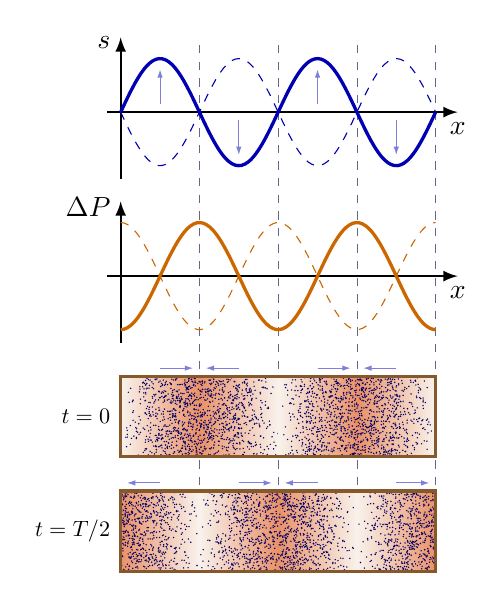
\begin{tikzpicture}
  \message{Standing wave plot...^^J}
  \def\lam{2.0}      % wavelength
  \def\n{2}          % harmonic
  \def\L{\n*\lam}    % length
  \def\ymax{0.85}    % y maximum
  \def\xmax{1.02*\L} % x maximum
  \def\A{0.80*\ymax} % amplitude
  \def\D{1.20*\ymax} % pipe diameter
  \def\s{2.45*\ymax} % shift
  \def\N{1200}       % number of points
  %\def\N{500}        % number of points
  
  % DISPLACEMENT
  \foreach \i [evaluate={\x=(\i-0.75)*\lam;}] in {1,...,\n}{
    \draw[myarr] (\x,0.15*\A) --++ (0,0.65*\A);
    \draw[myarr] (\x+\lam/2,-0.15*\A) --++ (0,-0.65*\A);
    \draw[blue!20!black!60,very thin,dashed] (\x+\lam/4,\ymax) --++ (0,-2.8*\s);
    \draw[blue!20!black!60,very thin,dashed] (\x+3*\lam/4,\ymax) --++ (0,-2.8*\s);
  }
  \draw[->,thick] (0,-\ymax) -- (0,0.1+\ymax) node[below=2,left] {$s$};
  \draw[->,thick] (-0.2*\ymax,0) -- (0.2+\xmax,0) node[below] {$x$};
  \draw[xcol,very thick,samples=100,smooth,variable=\x,domain=0:\L]
    plot(\x,{\A*sin(360/\lam*\x)});
  \draw[xcol,dashed,samples=100,smooth,variable=\x,domain=0:\L]
    plot(\x,{-\A*sin(360/\lam*\x)});
  
  % PRESSURE
  \begin{scope}[shift={(0,-\s)}]
    \draw[->,thick] (0,-\ymax) -- (0,0.1+\ymax) node[below=2,left] {$\Delta P$};
    \draw[->,thick] (-0.2*\ymax,0) -- (0.2+\xmax,0) node[below] {$x$};
    \draw[Pcol,very thick,samples=100,smooth,variable=\x,domain=0:\L]
      plot(\x,{\A*sin(360/\lam*\x-90)});
    \draw[Pcol,dashed,samples=100,smooth,variable=\x,domain=0:\L]
      plot(\x,{-\A*sin(360/\lam*\x-90)});
  \end{scope}
  
  % TUBE, t = 0
  \message{  Generating gas particles at t = 0...^^J}
  \begin{scope}[shift={(0,-2.1*\s)}]
    \fill[thin air] (0,0) rectangle++ (\L,\D); % to fill seams
    \foreach \i [evaluate={\x=(\i-1)*\lam;}] in {1,...,\n}{
      \draw[myarr] (\x+0.25*\lam,1.1*\D) --++ ( 0.21*\lam,0);
      \draw[myarr] (\x+0.75*\lam,1.1*\D) --++ (-0.21*\lam,0);
      \path[left color=thin air,right color=thin air,middle color=dense air]
        (\x,0) rectangle (\x+\lam,\D);
      \foreach \i in {1,...,\N}{
        \fill[blue!40!black] ({\x+acos(-rand)*\lam/180},{\D*(1+rand)/2}) circle(0.01);
      }
    }
    \draw[wood] (0,0) rectangle++ (\L,\D);
    \node[left=1,scale=0.8] at (0,\D/2) {$t=0$};
  \end{scope}
  
  % TUBE, t = T/2
  \message{  Generating gas particles at t = T/2...^^J}
  \begin{scope}[shift={(0,-2.8*\s)}]
    \fill[dense air] (0,0) rectangle++ (\L,\D); % to fill seams
    \foreach \i [evaluate={\x=(\i-1)*\lam;}] in {1,...,\n}{
      \draw[myarr] (\x+0.25*\lam,1.1*\D) --++ (-0.21*\lam,0);
      \draw[myarr] (\x+0.75*\lam,1.1*\D) --++ ( 0.21*\lam,0);
      \path[left color=dense air,right color=dense air,middle color=thin air]
        (\x,0) rectangle (\x+\lam,\D);
    }
    \foreach \i [evaluate={\x=(\i-2)*\lam;}] in {2,...,\n}{
      \foreach \i in {1,...,\N}{
        \fill[blue!40!black] ({\x+\lam/2+acos(-rand)*\lam/180},{\D*(1+rand)/2}) circle(0.01);
      }
    }
    \foreach \i in {1,...,\N}{
      \ifodd\i
        \fill[blue!40!black] ({acos(-(rand+1)/2)*\lam/180-\lam/2},{\D*(1+rand)/2}) circle(0.01);
      \else
        \fill[blue!40!black] ({\L+acos(-(rand-1)/2)*\lam/180-\lam/2},{\D*(1+rand)/2}) circle(0.01);
      \fi
    }
    \draw[wood] (0,0) rectangle++ (\L,\D);
    \node[left=1,scale=0.8] at (0,\D/2) {$t=T/2$};
  \end{scope}
  
\end{tikzpicture}


%%%%%%%%%%%%%%%%%%%%%%%%%%
% STANDING WAVE - CLOSED %
%%%%%%%%%%%%%%%%%%%%%%%%%%

% STANDING WAVE - CLOSED, n=1
\def\L{5.0} % pipe length
\def\R{0.6} % pipe radius
\def\wave#1{
  \message{Standing wave #1 (closed)..^^J}
  \pgfmathsetmacro\lam{2*\L/#1} % wavelength
  \clip (-0.1,-1.3*\R) rectangle (1.27*\L,1.1*\R); % same canvas size
  \fill[thin air] (0,-\R) rectangle (\L,\R);
  \foreach \i in {1,...,#1}{
    \path[left color=thin air,right color=dense air,
          opacity=0.3,shading angle={(2*\i+1)*90}]
      ({(\i-1)*\lam/2},-\R) rectangle++ (\lam/2,2*\R);
  }
  \draw[Pline,samples=100,smooth,variable=\x,domain=0:\L]
    plot(\x,{ (\R-0.041)*cos(360/(\lam)*\x)})
    plot(\x,{-(\R-0.041)*cos(360/(\lam)*\x)});
  \draw[wood] (-0.01,-\R) rectangle (\L+0.01,\R);
  %\draw[->,thick] (0,-1.2*\R) -- (0,0.2+1.2*\R) node[left] {$\Delta P$};
  %\draw[->,thick] (-0.2*\R,0) -- (0.2+\L,0) node[below] {$x$};
  %\path (0,-1.3*\R) rectangle (1.3*\L,1.1*\R); % same canvas size
}
\begin{tikzpicture}
  \draw[<->] (0,-1.3*\R) --++ (\L,0)
    node[midway,below=-4,fill=white,inner sep=0.5,scale=0.8] {$L=\lambda/2$};
  \wave{1}
  \node[right=2,align=left] at (\L,0) {$n=1$\\[1mm]$\lambda=2L$};
\end{tikzpicture}

% STANDING WAVE - CLOSED, n=2
\begin{tikzpicture}
  \wave{2}
  \node[right=2,align=left] at (\L,0) {$n=2$\\[1mm]$\lambda=L$};
\end{tikzpicture}

% STANDING WAVE - CLOSED, n=3
\begin{tikzpicture}
  \wave{3}
  \node[below=3,right=2,align=left] at (\L,0) {$n=3$\\[2mm]$\lambda=\dfrac{2L}{3}$};
\end{tikzpicture}

% STANDING WAVE - CLOSED, n=4
\begin{tikzpicture}
  \wave{4}
  \node[below=3,right=2,align=left] at (\L,0) {$n=4$\\[2mm]$\lambda=\dfrac{L}{2}$};
\end{tikzpicture}


%%%%%%%%%%%%%%%%%%%%%%%%%%%%%
% STANDING WAVE - HALF-OPEN %
%%%%%%%%%%%%%%%%%%%%%%%%%%%%%

% STANDING WAVE - HALF-OPEN, n=1
\def\wave#1{
  \message{Standing wave #1 (half-open)..^^J}
  \pgfmathsetmacro\lam{4*\L/(2*#1-1)} % wavelength
  \clip (-0.1,-1.3*\R) rectangle (1.27*\L,1.1*\R); % same canvas size
  \fill[thin air] (0,-\R) rectangle (\L,\R);
  \begin{scope}
    \clip (0,-\R) rectangle (\L,\R);
    \foreach \i in {1,...,#1}{
      \path[left color=thin air,right color=dense air,
            opacity=0.3,shading angle={(2*\i+1)*90}]
        ({(\i-1)*\lam/2},-\R) rectangle++ (\lam/2,2*\R);
    }
  \end{scope}
  \draw[Pline,samples=100,smooth,variable=\x,domain=0:\L]
    plot(\x,{ (\R-0.041)*cos(360/(\lam)*\x)})
    plot(\x,{-(\R-0.041)*cos(360/(\lam)*\x)});
  \draw[wood,line cap=round]
     (\L+0.01,\R) -| (-0.01,-\R) -- (\L+0.01,-\R);
  %\draw[->,thick] (0,-1.2*\R) -- (0,0.2+1.2*\R) node[left] {$\Delta P$};
  %\draw[->,thick] (-0.2*\R,0) -- (0.2+\L,0) node[below] {$x$};
}
\begin{tikzpicture}
  \draw[<->] (0,-1.3*\R) --++ (\L,0)
    node[midway,below=-4,fill=white,inner sep=0.5,scale=0.8] {$L=\lambda/4$};
  \wave{1}
  \node[right=2,align=left] at (\L,0) {$n=1$\\[1mm]$\lambda=4L$};
\end{tikzpicture}

% STANDING WAVE - HALF-OPEN, n=3
\begin{tikzpicture}
  \wave{2}
  \node[below=3,right=2,align=left] at (\L,0) {$n=3$\\[2mm]$\lambda=\dfrac{4L}{3}$};
\end{tikzpicture}

% STANDING WAVE - HALF-OPEN, n=5
\begin{tikzpicture}
  \wave{3}
  \node[below=3,right=2,align=left] at (\L,0) {$n=5$\\[2mm]$\lambda=\dfrac{4L}{5}$};
\end{tikzpicture}

% STANDING WAVE - HALF-OPEN, n=7
\begin{tikzpicture}
  \wave{4}
  \node[below=3,right=2,align=left] at (\L,0) {$n=7$\\[2mm]$\lambda=\dfrac{4L}{7}$};
\end{tikzpicture}


%%%%%%%%%%%%%%%%%%%%%%%%%%%%%
% STANDING WAVE - OPEN-OPEN %
%%%%%%%%%%%%%%%%%%%%%%%%%%%%%

% STANDING WAVE - OPEN-OPEN, n=1
\def\wave#1{
  \message{Standing wave #1 (open-open)..^^J}
  \pgfmathsetmacro\lam{2*\L/#1} % wavelength
  \clip (-0.1,-1.3*\R) rectangle (1.27*\L,1.1*\R); % same canvas size
  \fill[thin air] (0,-\R) rectangle (\L,\R);
  \begin{scope}
    \clip (0,-\R) rectangle (\L,\R);
    \foreach \i in {0,...,#1}{
      \path[left color=thin air,right color=dense air,
            opacity=0.3,shading angle={(2*\i+1)*90}]
        ({(\i-0.5)*\lam/2},-\R) rectangle++ (\lam/2,2*\R);
    }
  \end{scope}
  \draw[Pline,samples=100,smooth,variable=\x,domain=0:\L]
    plot(\x,{ (\R-0.041)*sin(360/(\lam)*\x)})
    plot(\x,{-(\R-0.041)*sin(360/(\lam)*\x)});
  \draw[wood,line cap=round]
    (-0.01, \R) -- (\L+0.01, \R)
    (-0.01,-\R) -- (\L+0.01,-\R);
  %\draw[->,thick] (0,-1.2*\R) -- (0,0.2+1.2*\R) node[left] {$\Delta P$};
  %\draw[->,thick] (-0.2*\R,0) -- (0.2+\L,0) node[below] {$x$};
}
\begin{tikzpicture}
  \draw[<->] (0,-1.3*\R) --++ (\L,0)
    node[midway,below=-4,fill=white,inner sep=0.5,scale=0.8] {$L=\lambda/2$};
  \wave{1}
  \node[right=2,align=left] at (\L,0) {$n=1$\\[1mm]$\lambda=2L$};
\end{tikzpicture}

% STANDING WAVE - OPEN-OPEN, n=2
\begin{tikzpicture}
  \wave{2}
  \node[right=2,align=left] at (\L,0) {$n=2$\\[2mm]$\lambda=L$};
\end{tikzpicture}

% STANDING WAVE - OPEN-OPEN, n=3
\begin{tikzpicture}
  \wave{3}
  \node[below=3,right=2,align=left] at (\L,0) {$n=3$\\[2mm]$\lambda=\dfrac{2L}{3}$};
\end{tikzpicture}

% STANDING WAVE - OPEN-OPEN, n=4
\begin{tikzpicture}
  \wave{4}
  \node[below=3,right=2,align=left] at (\L,0) {$n=4$\\[2mm]$\lambda=\dfrac{L}{2}$};
\end{tikzpicture}

\end{document}